\section{Microwind}

Microwind to zintegrowane oprogramowanie EDA (ang. \textit{Electronic Design Automation}),
które wspiera automatyzację procesu projektowania układów scalonych oraz płytek drukowanych.
%służące do automatyzacji procesu projektowania układów scalonych lub płytek drukowanych,
Program umożliwia projektowanie, symulacje, weryfikacje oraz testowanie układów elektronicznych~\cite{eda}.
Opracowany przez dra E. Sicarda do celów edukacyjnych,
w Tuluzie, Francja.
Sam program składa się z kilku modułów,
które wspierają różne etapy projektowania układów scalonych~\cite{Microwind}.
Instalacja w przypadku Microwinda jest prosta, wymaga jedynie pobrania pliku instalacyjnego z oficjalnej strony,
a następnie zainstalowania go na komputerze z systemem Windows~\cite{Microwind},
jest to natomiast wersja demonstracyjna, pełna wersja wymaga licencji.
Dostępna jest także archiwalna pełna wersja programu, która jest dostępna za darmo~\cite{old_microwind}.
Oficjalna strona udostępnia nie tylko instalatory, ale również dokumentację oraz przykłady projektów,
%Strona zawiera również dokumentację oraz przykłady projektów,
które mogą być wykorzystane w celach edukacyjnych~\cite{Microwind}.\\
\indent Jednym z kluczowych modułów programu Microwind jest \textbf{Nano Lambda},
do projektowania topografii układów scalonych.
Moduł ten uruchamia się automatycznie po włączeniu Microwinda.
%pojawiający się domyślnie po uruchomieniu programu.
%Posiada dość nieskomplikowany interfejs graficzny z paskiem menu i narzędzi
Interfejs graficzny edytora jest prosty i całkiem intuicyjny,
składa się z paska menu, narzędzi, obszaru roboczego oraz pływającego okna palety warstw,
co przedstawiono na rys.~\ref{fig:microwind_okno}.
Dzięki paskowi narzędzie oraz oknie palety warstw użytkownik ma szybki dostęp do większości funkcji programu,
przy czym należy zaznaczyć, że w porównaniu do Magica, ilość dostępnych warstw jest dużo mniejsza.
%oraz pływającym oknem palety warstw, przedstawiony na rys.~\ref{fig:microwind_okno}.

\begin{figure}[h]
    \centering
    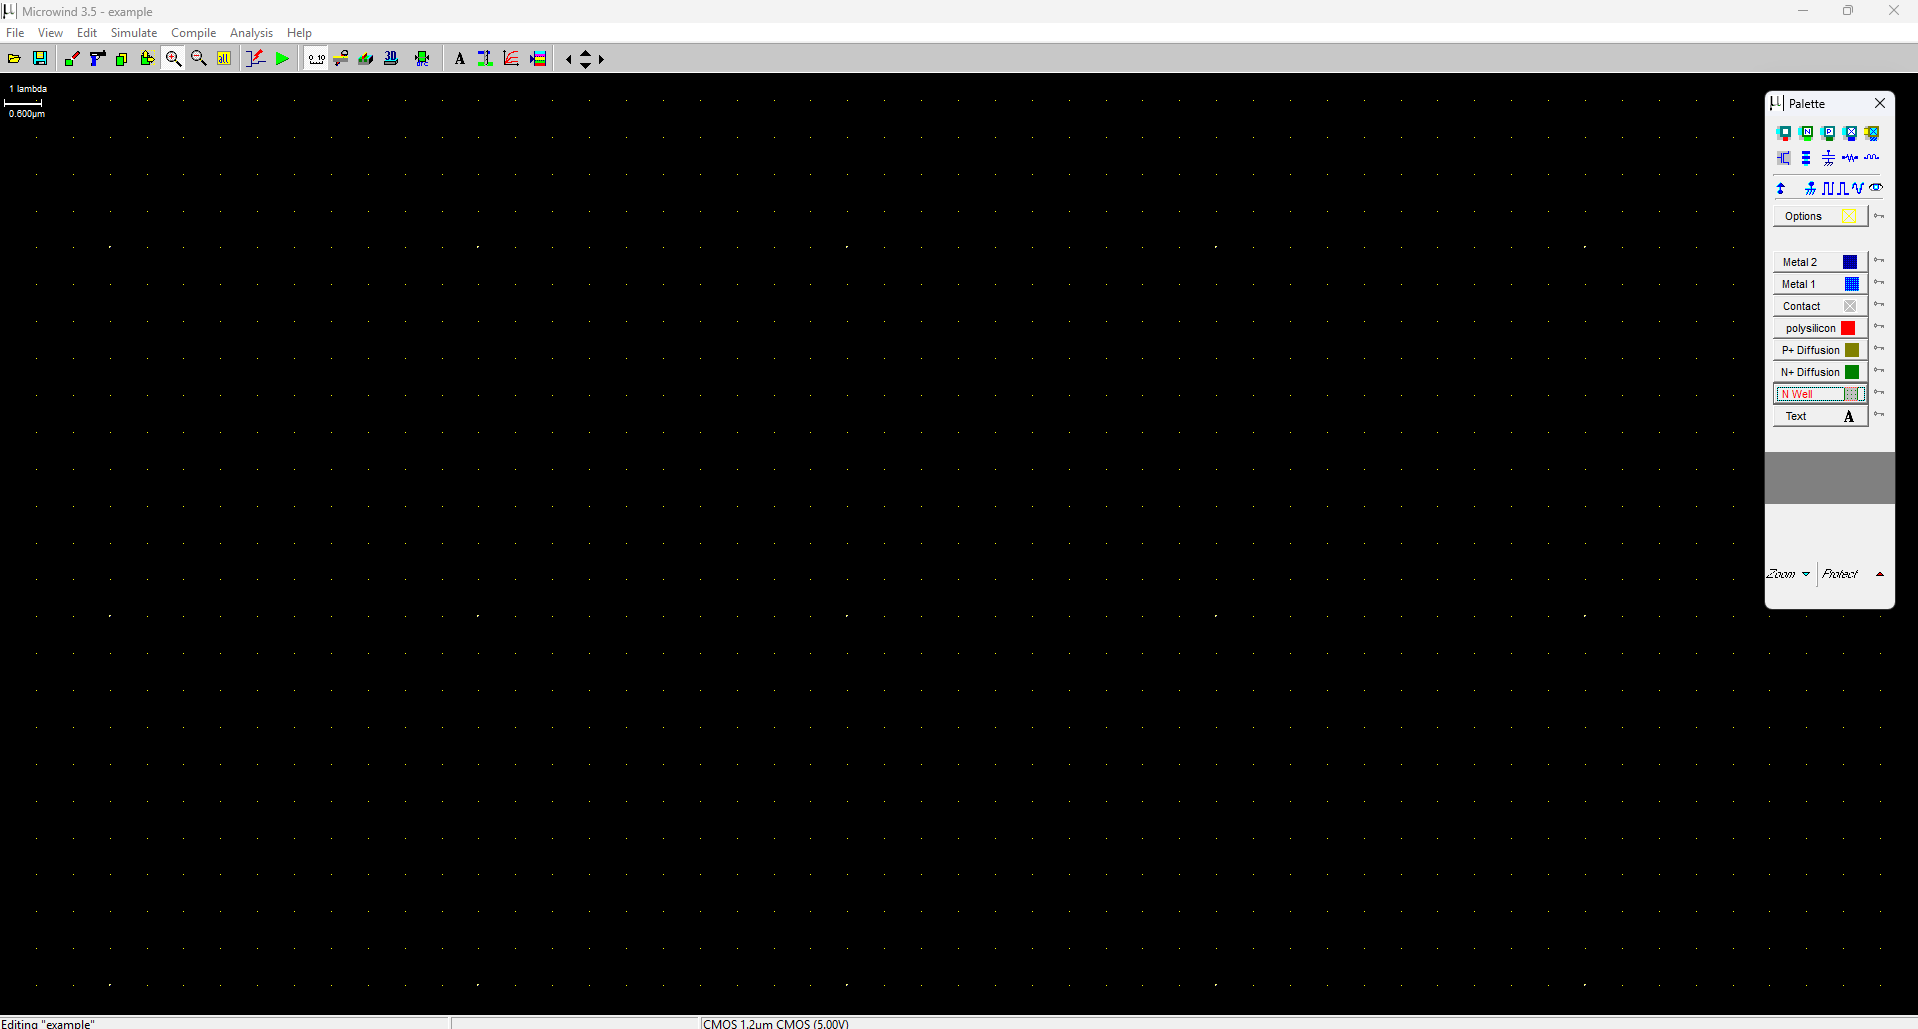
\includegraphics[width=.9\textwidth]{chapters/chapter2/img/microwind_okno}
    \caption[Widok głównego okna programu Microwind.]{Widok głównego okna programu Microwind, źródło:~\cite{Microwind}.}
    \label{fig:microwind_okno}
\end{figure}

\indent Rysowanie odbywa się w sposób zbliżony do klasycznych edytorów grafiki.
%poprzez wybór warstwy z palety,
Użytkownik wybiera warstwę z palety,
a następnie rysuje prostokątne komórki,
przeciągając kursor po obszarze roboczym przy wciśniętym lewym lub środkowym przycisku myszy. 
%a następnie przeciągając kursorem po obszarze roboczym przy wciśniętym lewym lub środkowym przycisku myszy,
%rysując przy tym prostokątną komórkę.
Nieznaczną wadą rysowania w Microwindzie jest brak przyciągania do siatki,
co utrudnia precyzyjne rozmieszczanie elementów.
%przez co jest mało precyzyjne.
Dodatkowo poruszanie się po obszarze roboczym wymaga używania klawiszy kierunkowych lub przycisków na pasku narzędzi,
co jest rozwiązaniem przestarzałym i mniej ergonomicznym w porównaniu do współczesnych standardów.
%Program Microwind, poza typowymi narzędziami edycji, charakteryzuje się wieloma zautomatyzowanymi narzędziami,
%pozwalającymi generowanie elementów schematów,
Program wyróżnia się jednak wieloma zautomatyzowanymi narzędziami,
które przykładowo umożliwiają generowanie elementów schematów na podstawie funkcji logicznych lub kodu Verilog~\cite{microwind_operation_commands}. 
%na przykład na podstawie funkcji logicznych lub kodu Verilog~\cite{microwind_operation_commands}.\\
Poza tym edytor schematów posiada wiele integracji z innymi modułami programu,
dzięki nim można na przykład:
\begin{citemize}
    \item na podstawie zaprojektowanego schematu obwodu elektrycznego, wygenerować topografię układu scalonego,
    \item zobaczyć kroki procesu technologicznego w 3D,
    \item zobaczyć przekrój układu scalonego,
    \item czy nawet wykonać symulacje na samym schemacie.
\end{citemize}
%\indent Ze względu na brak otwartego kodu źródłowego trudno określić dokładnie zastosowane mechanizmy edytora,
%natomiast na podstawie obserwacji można stwierdzić,
Warto zauważyć, że w celu ograniczenia zużycia pamięci program posiada limit liczby elementów w schemacie,
przedstawione na rys.

\begin{figure}[h]
    \centering
    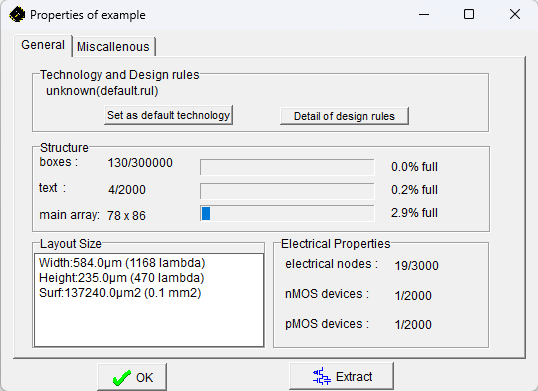
\includegraphics[width=.9\textwidth]{chapters/chapter2/img/microwind_opcje}
    \caption[Okno właściwości programu, ze wskazaniami zuzycia limitu elementów.]
    {
        Okno właściwości programu, ze wskazaniami zuzycia limitu elementów,
        źródło:~\cite{Microwind}.
    }
    \label{fig:microwind_limit}
\end{figure}

Brak otwartego kodu źródłowego programu Microwind uniemożliwia dokładne poznanie mechanizmów jego działania.
Na podstawie obserwacji można jednak zauważyć,
że każda edycja schematu wywołuje ponowne rysowanie całego obszaru roboczego,
na co wskazuje jego miganie, zauważalne w szczególności przy usuwaniu obszaru.\\
%Ta sama operacja również wskazuje na strukturę danych, która zakotwiczeniu komórek w kolumnach,
%ponieważ po usunięciu obszaru wewnątrz większej komórki, cała kolumna zostaje usunięta.\\
\indent Domyślna szata graficzna samego edytora charakteryzuje się wysokim kontrastem.
%gdzie warstwy są jednolitymi kolorami, częściowo przezroczystymi,
Większość z warstw jest przedstawiona jako jednolity kolor z częściową przezroczystością,
co pozwala na zauważenie nakładających się obszarów, przykład przedstawiono na rys.~\ref{fig:microwind_tran}.
%co jest zauważalne, gdy warstwy te się nakładają, przykład przedstawiono na rys.~\ref{fig:microwind_tran}.

\begin{figure}[h]
    \centering
    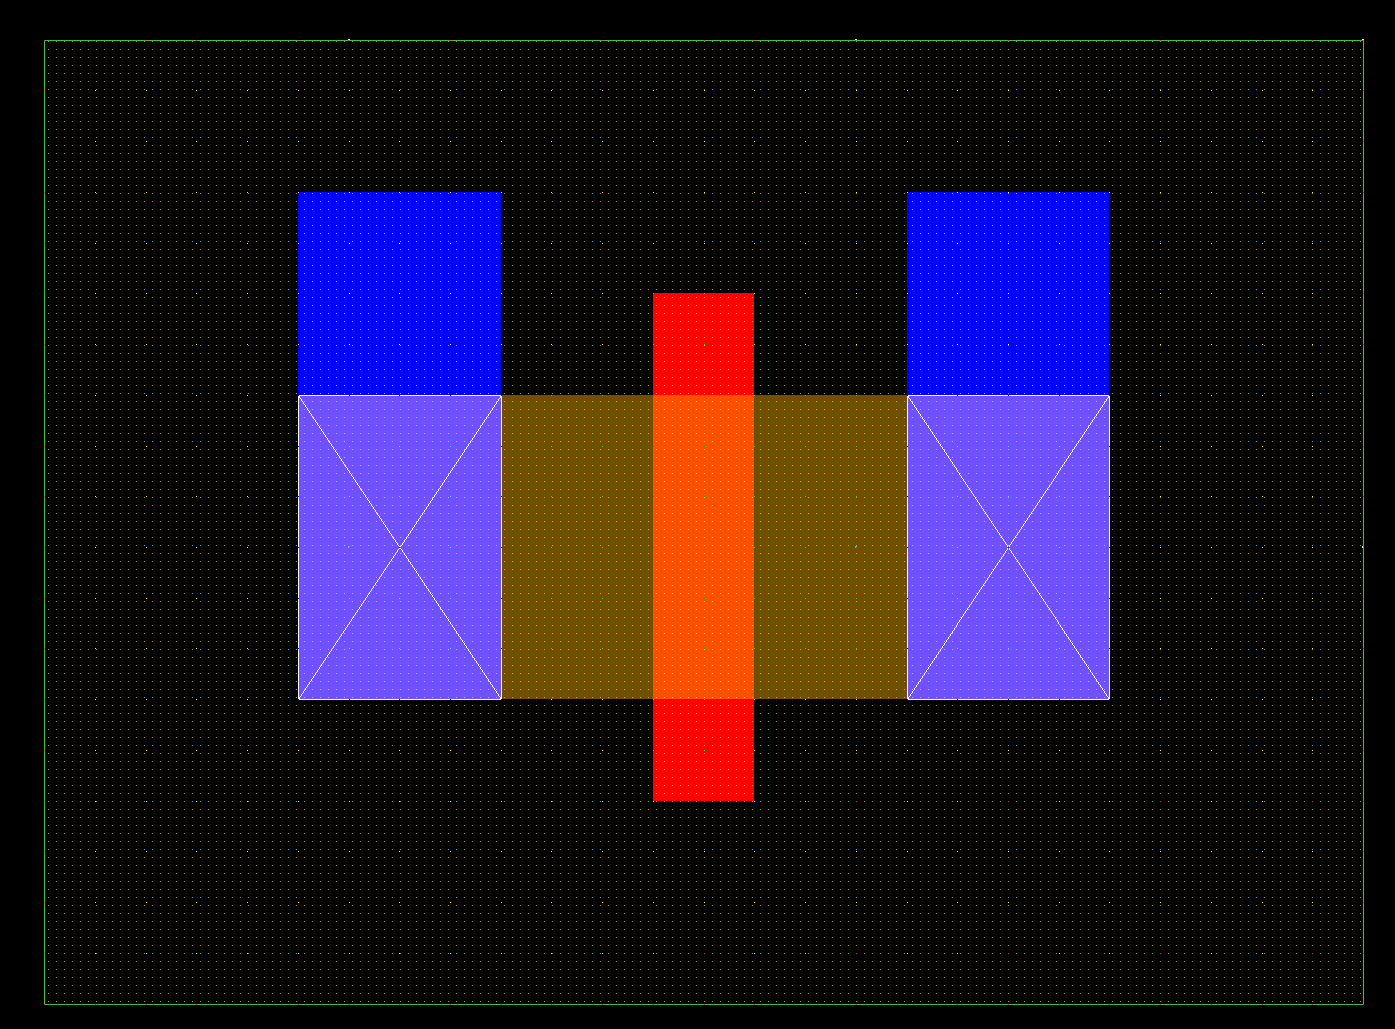
\includegraphics[width=.9\textwidth]{chapters/chapter2/img/microwind_tran}
    \caption[Przykład tranzystora narysowanego w programie Microwind.]
    {
        Przykład tranzystora narysowanego w programie Microwind,
        warstwy \textit{Metal 1}, \textit{P+ Diffusion} oraz \textit{Polysilicon} są jednoilitymi kolorami,
        wyjątkiem jest \textit{N Well},
        źródło: opracowanie własne.
    }
    \label{fig:microwind_tran}
\end{figure}

Tło edytora można zmienić na białe, przy czym warstwy zostają wtedy przedstawione za pomocą kolorowych wzorów,
pokazane na rys.~\ref{fig:microwind_biale}.
Dzięki temu widokowi można dostrzec, że każda rysowana komórka jest oddzielną instancją,
przez możliwe jest rysowanie komórek na sobie,
widoczne na rys.~\ref{fig:microwind_nadpisanie}, co nie jest optymalne w kwestii zużycia pamięci.
Dodatkowo motyw ten pozwala zobaczyć, że komórki są dzielone na kolumny,
gdy wycinany jest kawałek większej komórki przy każdorazowym wykonaniu tej operacji,
przykład czego przedstawiono na rys.~\ref{fig:microwind_kolumny}.

\begin{figure}[h]
    \centering
    \begin{subfigure}{.45\textwidth}
        \centering
        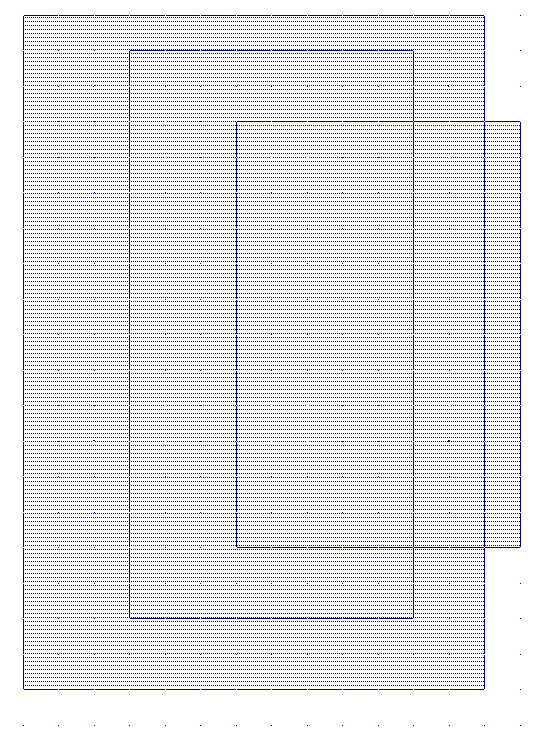
\includegraphics[width=.5\linewidth]{chapters/chapter2/img/microwind_nadpisanie}
        \caption{Komórki nakładające się na siebie.}
        \label{fig:microwind_nadpisanie}
    \end{subfigure}
    \begin{subfigure}{.45\textwidth}
        \centering
        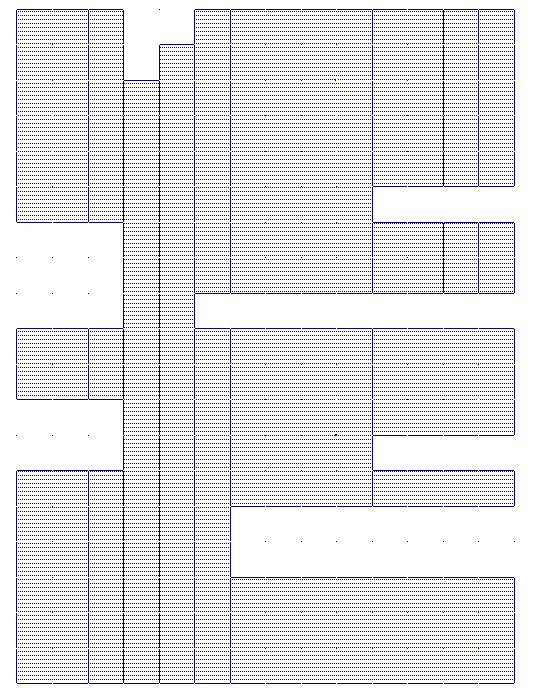
\includegraphics[width=.5\linewidth]{chapters/chapter2/img/microwind_kolumny}
        \caption{Komórki w formie kolumn.}
        \label{fig:microwind_kolumny}
    \end{subfigure}
    \caption[Losowo narysowane komórki warstwy \textit{Metal 2} na białym tle.]
    {
        Losowo narysowane komórki warstwy \textit{Metal 2} na białym tle,
        źródło: opracowanie własne.
    }
    \label{fig:microwind_biale}
\end{figure}

%\begin{figure}[h]
%    \centering
%    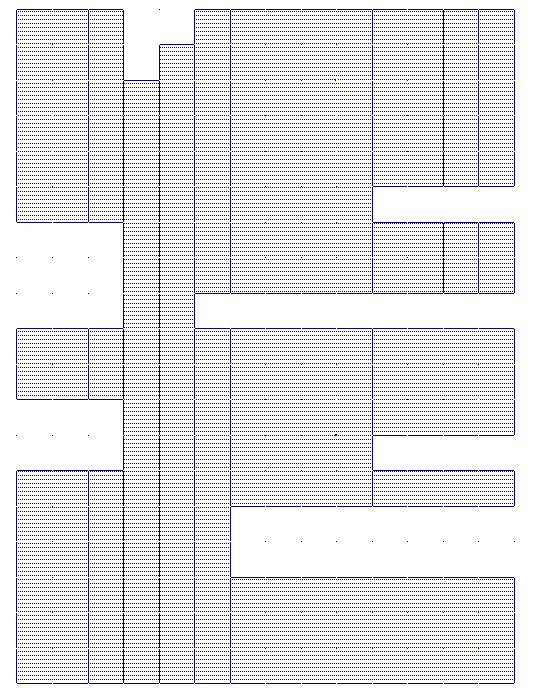
\includegraphics[width=.9\textwidth]{chapters/chapter2/img/microwind_kolumny}
%    \caption[Losowo narysowane komórki warstwy \textit{Metal 2} na białym tle.]
%    {
%        Losowo narysowane komórki warstwy \textit{Metal 2} na białym tle,
%        można rozróżnić każdą z komórek, nawet te nakładające się na siebie,
%        na czerwono zaznaczono obszar gdzie wycinano większą komórkę,
%        przez co zauważalne jest pojawienie się kolumn, źródło: opracowanie własne.
%    }
%    \label{fig:microwind_kolumny}
%\end{figure}
